\section{Desktop}

\subsection{GWC-Viewer}
Der GWC-Viewer (Abb. \ref{viewer_main}) ist ein Hilfsmittel um zu sehen, welche Objekte (Sounds, Bilder) (Abb. \ref{viewer_objects}) sich in dem Wherigo befinden. Diese kann man dann auch in den Ordner der Wherigo-Datei exportieren. Der LUA-Code (also das eigentliche Skript) ist compiliert und somit nicht lesbar, aber in einer späteren Version des GWC-Viewers wird dieser Code auch dekompiliert sein.

\begin{figure}[hb]
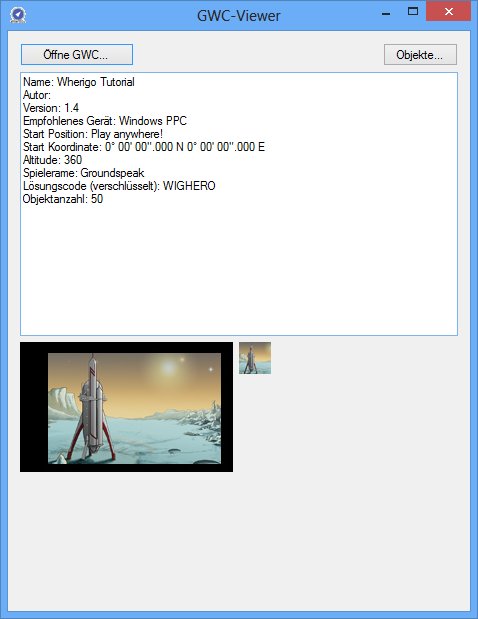
\includegraphics[width=0.4\textwidth]{screens/viewer_main}
\caption{GWC-Viewer Hauptfenster}
\label{viewer_main}
\end{figure}

\begin{figure}[hb]
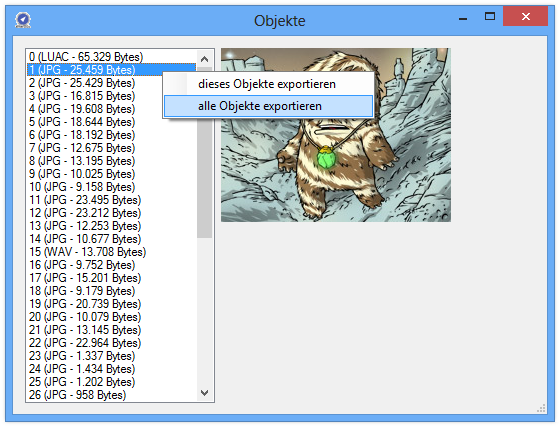
\includegraphics[width=0.4\textwidth]{screens/viewer_objects}
\caption{GCW-Viewer Objektansicht}
\label{viewer_objects}
\end{figure}


\subsection{LuaTester}
Mit dem LuaTester wird es möglich sein, eigene Lua-Skripte auszuführen. Derzeit ist dieser noch nicht als Download verfügbar.
